\chapter{连接杆}
\begin{figure}[htbp]
\centering
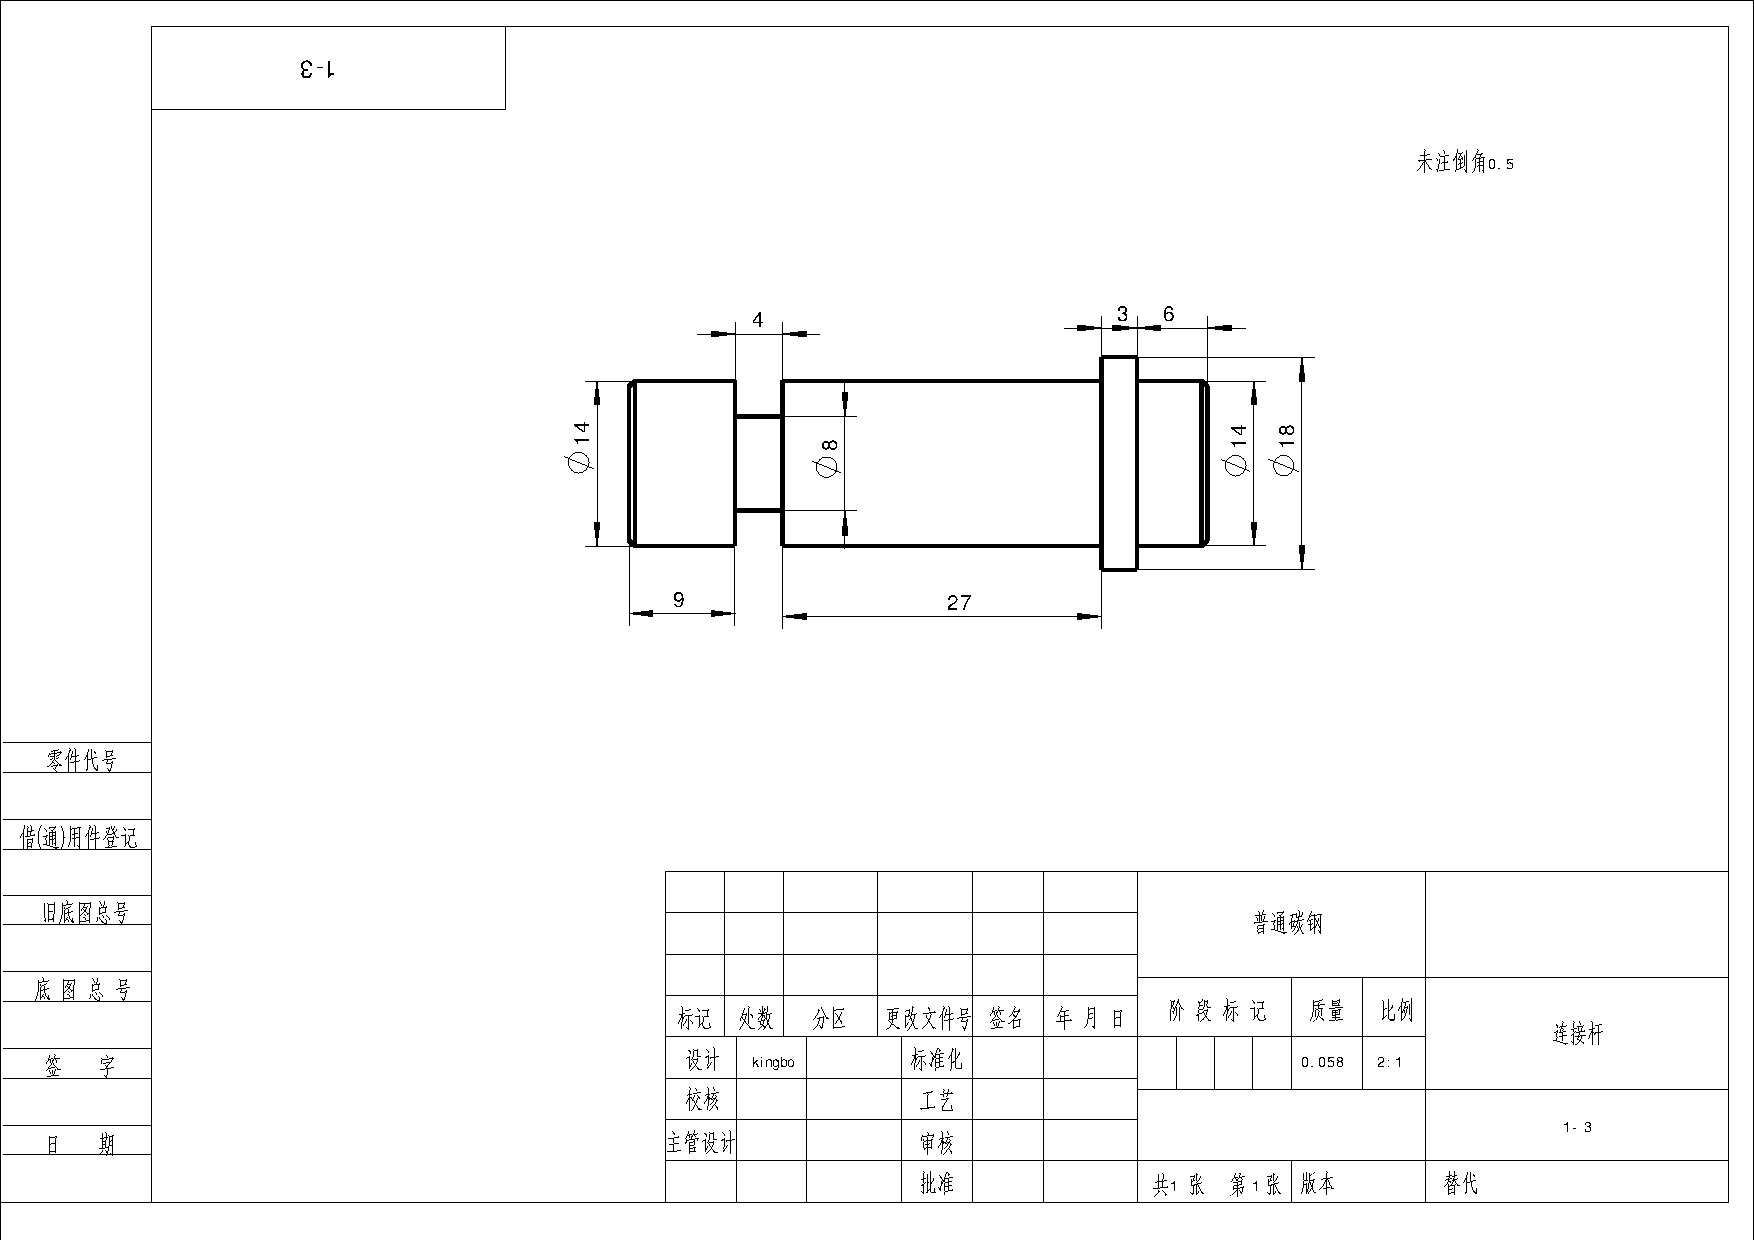
\includegraphics[scale=0.45]{xiaolunlianjiegan.pdf}
\caption{边接杆零件图}\label{fig:xiaolunlianjiegan}
\end{figure}

本章的目标是构建图\ref{fig:xiaolunlianjiegan}所示的小轮组连接杆零件的三维模型,并在此基础之上制作连接标杆的主视图、图纸图框和标题栏。因此本章重点讲解以下内容:
\begin{itemize}
\item 连接杆的三维模型构建
\item 块的定义和保存
\item 标题栏的制作
\item 线性尺寸标注
\item 文字标注
\end{itemize}


%\section{标题栏、尺寸、文字}

\endinput
\endinput